\usepackage{xcolor}
\usepackage{afterpage}
\usepackage{pifont,mdframed}
\usepackage[bottom]{footmisc}
\usepackage{multicol}

\makeatletter
\gdef\this@inputfilename{input.txt}
\gdef\this@outputfilename{output.txt}
\makeatother

\newcommand{\inputfile}{\texttt{input.txt}}
\newcommand{\outputfile}{\texttt{output.txt}}

\newenvironment{warning}
  {\par\begin{mdframed}[linewidth=2pt,linecolor=gray]%
    \begin{list}{}{\leftmargin=1cm
                   \labelwidth=\leftmargin}\item[\Large\ding{43}]}
  {\end{list}\end{mdframed}\par}

William è molto attento agli sprechi in casa: ogni volta che una spia o un display rimangono accesi, lui corre a spegnerli per risparmiare sulla bolletta. In certi casi è arrivato anche a scollegare i fili dei display meno essenziali (quello del videoregistratore, ad esempio) pur di evitare di lasciarli perennemente accesi. Purtroppo però, il suo \emph{contatore elettrico} è stato installato dal fornitore nazionale di energia, e sarebbe illegale manometterlo al fine di spegnergli il display! Il povero William quindi non può far altro che accettare di pagare una bolletta esorbitante a causa di questo display costantemente acceso.

Il contatore installato a casa di William presenta un \emph{display a sette segmenti}, lo stesso che si trova in molti tipi di radiosveglia. Questo tipo di display dispone di $7$ led per ciascuna cifra.

Nello schema di seguito si può vedere il numero di led richiesti per illuminare le varie cifre. Possiamo notare, ad esempio, che la cifra \texttt{1} richiede l'accensione di $2$ soli led, mentre la cifra \texttt{8} richiede che vengano accesi tutti e $7$:

\begin{center}
    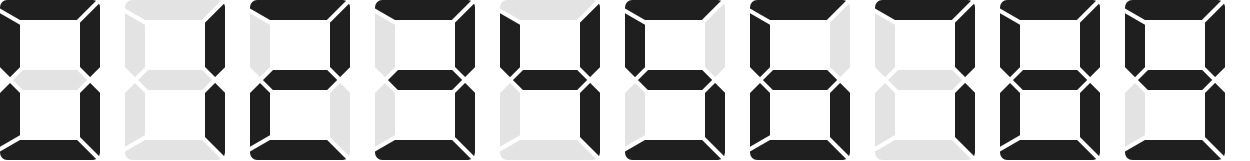
\includegraphics[width=0.6\linewidth]{7led}
\end{center}

All'inizio del mese il contatore verrà resettato a $0$ e, crescendo di $1$ alla volta a velocità costante, raggiungerà il valore $K$ alla fine del mese. Diciamo quindi che l'\emph{energia totale} consumata dal display è pari alla \emph{somma} dell'energia consumata per illuminare i numeri da $0$ a $K$. Per comodità, diremo inoltre che l'energia consumata per illuminare un singolo numero è pari al numero di led che è necessario illuminare per ciascuna delle sue cifre.

Ad esempio, per illuminare il solo numero \texttt{1234} servono $2+5+5+4 = 16$ unità di energia. William intende ora protestare presso l'agenzia elettrica per questo inaccettabile spreco, e vuole quindi sapere la somma delle unità consumate durante tutto il mese. Aiutalo scrivendo un programma che calcoli quanta energia verrà consumata per illuminare il display del contatore per tutta la durata del mese!


\Implementation
Dovrai sottoporre esattamente un file con estensione \texttt{.c}, \texttt{.cpp} o \texttt{.pas}.

\begin{warning}
Tra gli allegati a questo task troverai un template (\texttt{energia.c}, \texttt{energia.cpp}, \texttt{energia.pas}) con un esempio di implementazione da completare.
\end{warning}

Se sceglierai di utilizzare il template, dovrai implementare la seguente funzione:
\begin{center}\begin{tabularx}{\textwidth}{|c|X|}
\hline
C/C++  & \verb|long long int energia(long long int K);|\\
\hline
Pascal & \verb|function energia(K: int64): int64;|\\
\hline
\end{tabularx}\end{center}
In cui:
\begin{itemize}[nolistsep]
  \item L'intero $K$ rappresenta il valore che sarà scritto sul contatore alla fine del mese.
  \item La funzione dovrà restituire il numero di unità di energia consumate in totale dal display del contatore elettrico durante tutto il mese.
\end{itemize}
\pagebreak

\InputFile
Il file \inputfile{} è composto da un'unica riga contenente l'unico intero $K$.

\OutputFile
Il file \outputfile{} è composto da un'unica riga contenente un unico intero, la risposta a questo problema.

% Assunzioni
\Constraints
\begin{itemize}[nolistsep, itemsep=2mm]
	\item $0 \le K \le 1\,000\,000\,000\,000\,000$ ($10^{15}$).
	\item Non vengono illuminate cifre \texttt{0} non significative.
\end{itemize}

\Scoring
Il tuo programma verrà testato su diversi test case raggruppati in subtask.
Per ottenere il punteggio relativo ad un subtask, è necessario risolvere
correttamente tutti i test relativi ad esso.

\begin{itemize}[nolistsep,itemsep=2mm]
  \item \textbf{\makebox[2cm][l]{Subtask 1} [10 punti]}: Casi d'esempio.
  \item \textbf{\makebox[2cm][l]{Subtask 2} [30 punti]}: $K \leq 100$.
  \item \textbf{\makebox[2cm][l]{Subtask 3} [40 punti]}: $K \leq 1\,000\,000$.
  \item \textbf{\makebox[2cm][l]{Subtask 4} [20 punti]}: Nessuna limitazione specifica.
\end{itemize}

% Esempi
\Examples
\begin{example}
\exmpfile{energia.input0.txt}{energia.output0.txt}%
\exmpfile{energia.input1.txt}{energia.output1.txt}%
\exmpfile{energia.input2.txt}{energia.output2.txt}%
\end{example}


\Explanation
Nel \textbf{primo caso di esempio}, il contatore illuminerà i seguenti numeri:
\begin{multicols}{3}
\begin{itemize}[noitemsep]
    \item \texttt{0} ($6$ unità di energia)
    \item \texttt{1} ($2$ unità di energia)
    \item \texttt{2} ($5$ unità di energia)
    \item \texttt{3} ($5$ unità di energia)
\end{itemize}
\end{multicols}

Nel \textbf{secondo caso di esempio}, il contatore illuminerà i seguenti numeri:
\begin{multicols}{3}
\begin{itemize}[noitemsep]
    \item \texttt{0} ($6$ unità di energia)
    \item \texttt{1} ($2$ unità di energia)
    \item \texttt{2} ($5$ unità di energia)
    \item \texttt{3} ($5$ unità di energia)
    \item \texttt{4} ($4$ unità di energia)
    \item \texttt{5} ($5$ unità di energia)
    \item \texttt{6} ($6$ unità di energia)
    \item \texttt{7} ($3$ unità di energia)
    \item \texttt{8} ($7$ unità di energia)
    \item \texttt{9} ($6$ unità di energia)
    \item \texttt{10} ($2+6 = 8$ unità)
\end{itemize}
\end{multicols}
